% Chapter 4: Bộ lọc Kalman 7 trạng thái
\chapter{Bộ lọc Kalman 7 trạng thái}

Chương này trình bày thiết kế chi tiết khối ước lượng tư thế của \textbf{FC-v01} -- phần kết quả trung tâm của đề tài. Bộ lọc Kalman mở rộng (Extended Kalman Filter, EKF) là thuật toán hợp nhất số đo của nhiều cảm biến thành một ước lượng tư thế chắc chắn nhất, kèm theo con số đo mức độ chưa chắc chắn của ước lượng đó. EKF bảy trạng thái gồm quaternion tư thế (attitude) và độ lệch (bias) của con quay hồi tiếp (gyroscope, cảm biến đo tốc độ quay), với bước cập nhật quan sát (measurement update) giải tách thành các ma trận nhỏ cho gia tốc kế (cảm biến đo gia tốc) và từ kế (cảm biến la bàn) nhằm giảm chi phí tính toán trên ESP32. Ở tầng độ cao, một EKF ba trạng thái hợp nhất dữ liệu áp suất (barometer) và gia tốc kế để ước lượng tốc độ trục dọc. Khối ước lượng nằm trong tầng estimators của kiến trúc năm tầng (Hình~\ref{fig:rtos-arch}), nhận dữ liệu qua ring buffer từ tầng cảm biến.

\section{Vai trò của khối ước lượng trong chuỗi xử lý 500 Hz}

Trên \textbf{FC-v01}, chuỗi xử lý thời gian thực có tần suất cao nhất là 500 Hz và kết thúc tại khối ước lượng trạng thái (phần điều khiển độ bay còn được hoãn lại; phạm vi thực nghiệm trình bày trong chương kết quả). Do đó, chất lượng và độ trễ của khối EKF quyết định trực tiếp độ tin cậy của dữ liệu tư thế cung cấp cho đường telemetry BLE và bộ dữ liệu blackbox ghi trên thẻ nhớ.

Điểm khác biệt về mặt kiến trúc của \textbf{FC-v01} là việc tách EKF tư thế thành \textbf{hai tác vụ bất đồng bộ}: một tác vụ 500 Hz dự báo và cập nhật bằng gia tốc kế, một tác vụ 100 Hz cập nhật bằng từ kế, dùng chung một bộ máy EKF (engine) qua khóa mềm (mutex) \texttt{ekf\_state\_mutex} với thời hạn chờ 5~ms. Cách tổ chức này được phân tích chi tiết trong mục~\ref{sec:ekf-rtos}.

\section{Vector trạng thái (State Vector)}

\subsection{EKF tư thế bảy trạng thái (7-State Attitude EKF)}

Trạng thái của bộ lọc tư thế gồm hai thành phần:
\begin{equation}
\mathbf{x} = \left[\, \mathbf{q}^{T} \;\; \mathbf{b}_g^{T} \,\right]^{T} \in \mathbb{R}^{7}, \qquad
\mathbf{q} = \left[q_w, q_x, q_y, q_z\right]^{T}, \quad \mathbf{b}_g \in \mathbb{R}^{3},
\end{equation}
trong đó $\mathbf{q}$ là quaternion tư thế (đơn vị hóa, $|\mathbf{q}| = 1$) biểu diễn phép quay từ hệ trục thân (body frame) sang hệ trục chuẩn NED, và $\mathbf{b}_g$ là độ lệch (bias) ba trục của con quay hồi tiếp.

Đề tài chọn quaternion thay vì góc Euler làm biến trạng thái vì hai lý do: quaternion không gặp điểm kỳ dư (singularity) ở bất kỳ tư thế nào, và phép quay tổng hợp bằng tích quaternion chỉ cần các phép nhân và cộng số thực, phù hợp cho việc số hóa hiệu quả trên vi điều khiển~\cite{sola2017}. Nhược điểm --vector trạng thái có ràng buộc $|\mathbf{q}|=1$-- được xử lý bằng cách chuẩn hóa lại quaternion sau mỗi bước cập nhật đo (mục~\ref{sec:ekf-seq}). Ba trạng thái bias của con quay được mô hình hóa như một quá trình trôi chậm (random walk) và được ước lượng trực tuyến, giúp bộ lọc tự bù phần trôi của cảm biến giữa các lần hiệu chuẩn.

\subsection{EKF độ cao ba trạng thái (3-State Altitude EKF)}

Khối ước lượng độ cao dùng một EKF độc lập với vector trạng thái
\begin{equation}
\mathbf{x}_a = \left[\, z \;\; v_z \;\; b_a \,\right]^{T} \in \mathbb{R}^{3},
\end{equation}
gồm độ cao $z$ (suy ra từ áp suất khí quyển), vận tốc trục dọc $v_z$ và độ lệch trục dọc của gia tốc kế $b_a$. Thiết kế này được trình bày gọn ở mục~\ref{sec:ekf-alt}.

\section{Mô hình dự báo (predict)}

\subsection{Phương trình động học quaternion}

Gia tốc kế ba trục sau khi lọc thông thấp (mục~\ref{sec:ekf-calib}) cung cấp tốc độ góc $\boldsymbol\omega_m$; sau khi trừ đi ước lượng bias hiện tại $\mathbf{b}_g$, tốc độ góc thực $\boldsymbol\omega = \boldsymbol\omega_m - \mathbf{b}_g$ được tích phân vào quaternion theo phương trình động học liên tục:
\begin{equation}
\dot{\mathbf{q}} = \frac{1}{2}\, \mathbf{q} \otimes \begin{bmatrix} 0 \\ \boldsymbol\omega \end{bmatrix},
\label{eq:qkin}
\end{equation}
với $\otimes$ là tích quaternion. Rời rạc hóa với chu kỳ lấy mẫu $T_s = 2$~ms (tần suất 500 Hz) và giả thiết tốc độ góc gần không đổi trong một chu kỳ, khai triển Taylor bậc nhất của (\ref{eq:qkin}) cho phép chuyển trạng thái dưới dạng nhân ma trận tuyến tính~\cite{ahrs-ekf}:
\begin{equation}
\mathbf{q}_{k|k-1} = \mathbf{A}_k\, \mathbf{q}_{k-1|k-1}, \qquad
\mathbf{A}_k = \mathbf{I}_4 + \dfrac{T_s}{2}\, \boldsymbol\Omega(\boldsymbol\omega),
\label{eq:qupdate}
\end{equation}
trong đó $\boldsymbol\Omega(\boldsymbol\omega)$ là ma trận $4\times 4$ chống đối xứng của vector tốc độ góc:
\begin{equation}
\boldsymbol\Omega(\boldsymbol\omega) =
\begin{bmatrix}
0 & -\omega_x & -\omega_y & -\omega_z \\
\omega_x & 0 & \omega_z & -\omega_y \\
\omega_y & -\omega_z & 0 & \omega_x \\
\omega_z & \omega_y & -\omega_x & 0
\end{bmatrix}.
\end{equation}
Cách viết này cho phép tích phân tư thế bằng đúng một lệnh nhân ma trận $4\times 4$ qua tầng SIMD (một lệnh xử lý nhiều số cùng lúc, mục~\ref{sec:ekf-simd}), không cần dựng ma trận quay đầy đủ.

\subsection{Mô hình nhiễu và bước dự báo}

Bias con quay được mô hình hóa trôi chậm:
\begin{equation}
\mathbf{b}_{g,k} = \mathbf{b}_{g,k-1} + \mathbf{w}_{b,k}, \qquad \mathbf{w}_{b,k} \sim \mathcal{N}(0,\, \sigma_b^2 T_s\, \mathbf{I}_3).
\end{equation}
Khác với biến thể trạng thái-lỗi (error-state) phổ biến trong tài liệu~\cite{sola2017}, bộ lọc của \textbf{FC-v01} lan truyền trực tiếp Jacobi $7\times 7$ của hàm chuyển trạng thái $\mathbf{f}(\mathbf{x}) = \left[\left(\mathbf{A}_k\mathbf{q}\right)^{T} \;\; \mathbf{b}_g^{T}\right]^{T}$ theo toàn bộ vector trạng thái:
\begin{equation}
\mathbf{F} =
\begin{bmatrix}
\mathbf{A}_k & \mathbf{G}_b \\
\mathbf{0}_{3\times 4} & \mathbf{I}_3
\end{bmatrix},
\label{eq:F}
\end{equation}
trong đó khối trên-trái đúng bằng ma trận chuyển tiếp quaternion $\mathbf{A}_k$ ở (\ref{eq:qupdate}), còn $\mathbf{G}_b \in \mathbb{R}^{4\times 3}$ là đạo hàm riêng của $\mathbf{q}_{k|k-1}$ theo bias: vì $\boldsymbol\omega = \boldsymbol\omega_m - \mathbf{b}_g$, mỗi thành phần bias tác động ngược dấu tốc độ góc, $\mathbf{G}_b = -\tfrac{T_s}{2}\,\partial\bigl(\boldsymbol\Omega(\boldsymbol\omega)\mathbf{q}\bigr)/\partial\boldsymbol\omega$, được viết theo thành phần quaternion hiện tại:\begin{equation}
\dfrac{2}{T_s}\,\mathbf{G}_b =
\begin{bmatrix}
q_1 & q_2 & q_3 \\
-q_0 & q_3 & -q_2 \\
-q_3 & -q_0 & q_1 \\
q_2 & -q_1 & -q_0
\end{bmatrix}.
\end{equation}
Từ đó
\begin{equation}
\mathbf{P}_{k|k-1} = \mathbf{F}\, \mathbf{P}_{k-1|k-1}\, \mathbf{F}^{T} + \mathbf{Q}.
\end{equation}
Ma trận hiệp phương sai quá trình $\mathbf{Q}$ là ma trận chéo gồm hai thành phần: phương sai nhiễu quy về quaternion (từ nhiễu đo của con quay, bị tích phân trong pha dự báo) và phương sai trôi của bias -- hai nguồn bất định của pha dự báo.

\section{Cập nhật quan sát tuần tự (sequential update)}
\label{sec:ekf-seq}

\subsection{Ý tưởng giải tách cập nhật quan sát (Splitting the Measurement Update)}

Với bộ lọc chuẩn, hợp nhất hai nguồn đo khác tần suất đòi hỏi nghịch đảo một ma trận hiệp phương sai khối lớn, với chi phí tỷ lệ $n^3$ theo số chiều trạng thái $n$. Trên ESP32-S3 với dung lượng CPU hạn chế, đề tài áp dụng \textbf{cập nhật tuần tự}: gia tốc kế và từ kế được cập nhật thành hai bước độc lập, mỗi bước dùng một ma trận quan sát mỏng $3\times 7$ và chỉ nghịch đảo một ma trận hiệp phương sai phần dư cỡ $3\times 3$; về mặt đại số, hai cập nhật tuần tự với hiệp phương sai đo chéo nhau bằng không tương đương một cập nhật khối. Chi phí giảm đáng kể vì các ma trận nghịch đảo nhỏ hơn nhiều và mỗi bước chỉ chạy khi nguồn đo tương ứng sẵn sàng.

\subsection{Cập nhật gia tốc kế (đo trọng lực) (Accelerometer Update)}

Khi gia tốc kế đo được vector $\mathbf{a}_m$ và độ lớn của nó nằm trong vùng tin cậy, vector đo hướng được chuẩn hóa; vùng tin cậy loại trừ các đoạn gia tốc mạnh, khi vector đo không còn ưu thế lên phương trọng lực:
\begin{equation}
\hat{\mathbf{a}} = \frac{\mathbf{a}_m}{|\mathbf{a}_m|}.
\end{equation}
Mô hình quan sát là vector trọng lực \textit{dự báo} trong hệ trục thân, viết trực tiếp theo thành phần quaternion~\cite{sabatini2011}:
\begin{equation}
\mathbf{h}_a(\mathbf{q}) =
\begin{bmatrix}
2(q_1 q_3 - q_0 q_2) \\
2(q_0 q_1 + q_2 q_3) \\
q_0^{2} - q_1^{2} - q_2^{2} + q_3^{2}
\end{bmatrix}.
\end{equation}
Phần dư đo (innovation) là hiệu vector $\mathbf{y}_a = \hat{\mathbf{a}} - \mathbf{h}_a(\mathbf{q})$; nói cách khác, phần dư đo là hiệu giữa số đo thực tế và số đo dự báo. Ma trận quan sát là Jacobi $3\times 7$ đầy đủ $\mathbf{H}_a = \partial \mathbf{h}_a / \partial \mathbf{x}$, viết trực tiếp theo thành phần quaternion; ba cột về bias bằng không vì gia tốc kế không nhìn thấy bias con quay. Bước cập nhật Kalman chuẩn~\cite{kalman1960}:
\begin{equation}
\begin{aligned}
\mathbf{S}_a &= \mathbf{H}_a \mathbf{P}_{k|k-1} \mathbf{H}_a^{T} + \mathbf{R}_a, &
\mathbf{K}_a &= \mathbf{P}_{k|k-1} \mathbf{H}_a^{T} \mathbf{S}_a^{-1}, \\
\mathbf{x}_{k|k} &= \mathbf{x}_{k|k-1} + \mathbf{K}_a\, \mathbf{y}_a, &
\mathbf{P}_{k|k} &= (\mathbf{I} - \mathbf{K}_a \mathbf{H}_a)\,\mathbf{P}_{k|k-1}.
\end{aligned}
\end{equation}
trong đó chỉ có ma trận $\mathbf{S}_a$ cỡ $3\times 3$ cần nghịch đảo; quaternion được chuẩn hóa ngay sau cập nhật. Toàn bộ phép toán đi qua tầng SIMD nên chi phí mỗi lần cập nhật rất thấp.

\subsection{Cập nhật từ kế (đo hướng từ trường) (Magnetometer Update)}

Từ kế, sau khi hiệu chuẩn (mục~\ref{sec:ekf-calib}) và chuẩn hóa về độ dài đơn vị $|\mathbf{m}| = 1$, được hợp nhất theo cùng lược đồ với gia tốc kế. Vector từ trường trong hệ chuẩn được cấu hình dưới dạng hai hằng số $\mathbf{m}^{n} = \left[\,b_x \;\; 0 \;\; b_z\,\right]^{T}$. Vector dự báo trong hệ thân $\mathbf{h}_m(\mathbf{q}) = \mathbf{R}(\mathbf{q})^{T}\,\mathbf{m}^{n}$, phần dư đo $\mathbf{y}_m = \hat{\mathbf{m}} - \mathbf{h}_m(\mathbf{q})$ và ma trận Jacobi $3\times 7$ $\mathbf{H}_m$ được dùng trong cùng công thức cập nhật như trên.

Cập nhật từ kế \textbf{không} cần chạy 500~Hz vì từ trường địa phương biến đổi chậm; đề tài đặt nó ở tác vụ 100~Hz độc lập -- đây là lý do tồn tại hai tác vụ được phân tích ở mục~\ref{sec:ekf-rtos}.

\section{EKF độ cao (Altitude EKF)}
\label{sec:ekf-alt}

EKF độ cao ba trạng thái hợp nhất hai nguồn đo trên trục dọc: áp suất khí quyển (chậm nhưng không trôi) và tích phân gia tốc kế (nhanh nhưng trôi do $b_a$). Trạng thái được dự báo bằng phương trình chuyển động $\dot{z} = v_z$, $\dot{v}_z = a_z - b_a$ với bias trôi chậm, còn pha cập nhật là một bước vô hướng theo đo áp suất. Điểm đặc thù là \textbf{khởi tạo hiệp phương sai $\mathbf{P}_0$ trên mặt đất}: hiệp phương sai của bias được đặt nhỏ nhất trong ba trạng thái vì bias đã được hiệu chuẩn tĩnh trước bay (mục~\ref{sec:ekf-calib}); khả năng bám trôi khi bay do $\mathbf{Q}_a$ đảm bảo (mục~\ref{subsec:ekf-alt-init}).

\subsection{Mô hình dự báo của bộ lọc độ cao (Altitude Filter Prediction Model)}

Với chu kỳ lấy mẫu $T_s = 10$~ms (tần suất 100 Hz), vector trạng thái $\mathbf{x}_a = \left[z \;\; v_z \;\; b_a\right]^{T}$ được lan truyền bởi mô hình chuyển động rời rạc:
\begin{equation}
\mathbf{x}_{a,k|k-1} =
\begin{bmatrix}
1 & T_s & -\dfrac{T_s^{2}}{2} \\[4pt]
0 & 1   & -T_s \\[2pt]
0 & 0   & 1
\end{bmatrix}
\mathbf{x}_{a,k-1|k-1} +
\begin{bmatrix}
\dfrac{T_s^{2}}{2} \\[4pt]
T_s \\[2pt]
0
\end{bmatrix}
a_{z,k},
\label{eq:alt-predict}
\end{equation}
trong đó $a_{z,k}$ là gia tốc trục dọc theo hệ chuẩn, chiếu từ gia tốc kế đo trong hệ thân bằng quaternion tư thế do EKF tư thế cung cấp, và được coi như đầu vào điều khiển (control input) của mô hình -- gia tốc kế đo \textit{gia tốc riêng} (specific force) nên phần trôi $b_a$ phải nằm trong trạng thái thay vì vế nhiễu. Ma trận hiệp phương sai quá trình $\mathbf{Q}_a$ gộp nhiễu của gia tốc kế (nhiễu trắng bị tích phân thành trôi ngẫu nhiên trong $v_z$ và $z$) và tốc độ trôi của $b_a$:
\begin{equation}
\mathbf{P}_{a,k|k-1} = \mathbf{F}_a\, \mathbf{P}_{a,k-1|k-1}\, \mathbf{F}_a^{T} + \mathbf{Q}_a.
\end{equation}

\subsection{Cập nhật đo áp suất và vai trò bù trôi của bias (Pressure Update and Bias Drift Compensation)}

Bước cập nhật dùng duy nhất một nguồn đo: áp suất khí quyển đo được $p_k$ (Pa). Quan hệ áp suất -- độ cao là phi tuyến theo mô hình barometric chuẩn~\cite{bmp180}:
\begin{equation}
h(\mathbf{x}_a) = p_0 \left(1 - \dfrac{z}{44\,330}\right)^{5.255},
\end{equation}
với $p_0$ là áp suất tham chiếu mặt đất do FSM đặt khi hệ thống ở trạng thái \texttt{READY}. Vì mô hình quan sát phi tuyến, bộ lọc tuyến tính hóa tại điểm dự báo: ma trận quan sát $\mathbf{H}_a = \left[\,H_0 \;\; 0 \;\; 0\,\right]$ với
\begin{equation}
H_0 = \dfrac{\partial h}{\partial z} = -\dfrac{5.255\, p_0}{44\,330} \left(1 - \dfrac{z}{44\,330}\right)^{4.255} \quad (\text{Pa/m})
\end{equation}
được tính bằng đạo hàm riêng tại mỗi chu kỳ. Nhiễu đo của barometer nhỏ, nhưng bị ảnh hưởng bởi biến động khí áp thời tiết và dòng gió qua ống đo; nhiễu này được mô hình hóa bằng nhiễu Gauss $r_b$ (Pa\textsuperscript{2}). Phần dư đo (innovation) theo đơn vị áp suất là
\begin{equation}
y_k = p_k - h\bigl(\mathbf{x}_{a,k|k-1}\bigr),
\end{equation}
phương sai phần dư $S_k = H_0^{2}\, \mathbf{P}_{a,(0,0)} + r_b$, hệ số Kalman và bước cập nhật:
\begin{equation}
\mathbf{K}_k = \dfrac{H_0}{S_k}
\begin{bmatrix} \mathbf{P}_{a,(0,0)} & \mathbf{P}_{a,(1,0)} & \mathbf{P}_{a,(2,0)} \end{bmatrix}^{T},
\qquad
\mathbf{x}_{a,k|k} = \mathbf{x}_{a,k|k-1} + \mathbf{K}_k\, y_k,
\end{equation}
trong đó ước lượng bias được kẹp biên trong $\pm 2$~m/s\textsuperscript{2} để bảo đảm ổn định số học, và hiệp phương sai được cập nhật dạng $(\mathbf{I} - \mathbf{K}_k \mathbf{H}_a)\mathbf{P}_a$. Lợi ích của hợp nhất nằm ở hai thành phần \textit{không được đo trực tiếp}: $v_z$ và $b_a$ được ước lượng gián tiếp qua ma trận hiệp phương sai $\mathbf{P}_a$. Trên thực tế cơ chế này hoạt động như một \textbf{bộ bù trôi}: khi bias $b_a$ làm $v_z$ tích phân sai lệch dần, áp suất dự báo tách khỏi áp suất đo, và phần dư $y_k$ tích lũy qua các chu kỳ khiến $\mathbf{K}_k$ kéo các trạng thái về phía giá trị giải thích được phần tách đó -- barometer đóng vai trò ``mỏ neo'' dài hạn chặn trôi của tích phân gia tốc kế, trong khi gia tốc kế cung cấp độ phân giải tần số cao mà barometer không có. Vòng lặp dự báo--cập nhật này chạy độc lập ở 100 Hz và chỉ dùng các phép toán vô hướng và $3\times 3$, nên chi phí tính toán của bộ lọc là không đáng kể so với EKF tư thế.

\subsection{Vòng đời khởi tạo trên mặt đất (Ground Initialization)}
\label{subsec:ekf-alt-init}

Điều kiện khởi tạo $\mathbf{P}_0$ trên mặt đất gồm hai thời điểm. Khi hệ thống khởi động, bộ lọc được reset về $\mathbf{x}_a = \left[0 \;\; 0 \;\; 0\right]^{T}$ với $\mathbf{P}_0 = 0.1\,\mathbf{I}_3$, trong đó thành phần $(2,2)$ -- hiệp phương sai của $b_a$ -- được giảm xuống $0.01$, tức \textit{nhỏ nhất} trong ba trạng thái: bias đã được hiệu chuẩn tĩnh trước bay (mục~\ref{sec:ekf-calib}) nên dư lượng rất nhỏ; nếu khởi tạo hiệp phương sai lớn, bộ lọc sẽ đuổi theo nhiễu baro để ``tìm'' một trôi không tồn tại. Khi FSM chuyển sang \texttt{READY}, áp suất mặt đất ổn định được lấy làm tham chiếu $p_0$ và trạng thái $z$, $v_z$ đưa về 0 với hiệp phương sai $0.1$, xóa hiệp phương sai chéo $(z, v_z)$, giữ nguyên hiệp phương sai của bias. Mỗi bước dự báo, $\mathbf{Q}_a$ làm hiệp phương sai của $b_a$ tăng dần theo mô hình trôi chậm, nhờ đó hệ số Kalman vẫn phân bổ được phần dư đo về bias khi trôi thật xuất hiện khi bay.

Điểm khác biệt về mặt kỹ thuật so với EKF tư thế: EKF độ cao là \textbf{bộ lọc gọn trong một tác vụ} (thread-confined). Chỉ duy nhất tác vụ \texttt{EKF\_ALTITUDE} 100 Hz truy cập trạng thái, không cần khóa mềm; một nguồn dữ liệu đơn giản không đáng để đánh đổi chi phí khóa.

\section{Triển khai thời gian thực trên ESP32-S3 (Real-Time Implementation on ESP32-S3)}
\label{sec:ekf-rtos}

\subsection{Hai tác vụ bất đồng bộ dùng chung bộ máy EKF (Two Asynchronous Tasks Sharing the EKF Engine)}

Bảng~\ref{tab:ekf-tasks} tóm tắt cấu hình hai tác vụ EKF tư thế và một tác vụ EKF độ cao trong dự án, bổ sung vào bảng tác vụ tổng thể của chương trước (bảng~\ref{tab:tasks}).

\begin{table}[H]
\centering
\caption{Tác vụ ước lượng trạng thái trong \textbf{FC-v01}}
\label{tab:ekf-tasks}
\small
\begin{tabular}{@{}llcll@{}}
\toprule
\textbf{Tác vụ} & \textbf{Tần suất} & \textbf{Ưu tiên} & \textbf{Nhiệm vụ} & \textbf{Đồng bộ} \\
\midrule
\texttt{EKF\_ROLL\_PITCH} & 500 Hz & 3 & dự báo + cập nhật gia tốc kế & mutex \\
\texttt{EKF\_YAW}         & 100 Hz & 2 & cập nhật từ kế               & mutex \\
\texttt{EKF\_ALTITUDE}    & 100 Hz & 2 & hợp nhất baro + gia tốc kế   & không khóa \\
\bottomrule
\end{tabular}
\end{table}

Việc tách cập nhật từ kế sang tác vụ riêng nhằm giải quyết mâu thuẫn giữa hai yêu cầu: pha dự báo cần tần suất cao để tích phân con quay chính xác, trong khi cập nhật từ kế tốn chi phí tính toán hơn nhưng chỉ cần tần suất thấp. Hai tác vụ đều được cấu hình \texttt{tskNO\_AFFINITY}, tức là \textbf{phân tách theo tần suất trên bộ lập lịch SMP chứ không ghim lõi (core pinning)}. Hai tác vụ truy cập bộ máy dùng chung qua \texttt{ekf\_state\_mutex} với thời hạn chờ 5~ms; nếu không nhận được khóa, tác vụ từ kế bỏ qua chu kỳ hiện tại -- mất mát một chu kỳ được chấp nhận vì từ trường biến đổi chậm. Cả hai tác vụ nhận dữ liệu cảm biến qua ring buffer từ tầng tiền xử lý (bảng~\ref{tab:ipc}) và phát marker truy vết SystemView cho phép đo thời gian thực thi thực tế (trình bày trong chương kết quả).

\subsection{Vị trí bộ nhớ của trạng thái EKF (Memory Placement of the EKF State)}

Trạng thái EKF tư thế \texttt{AttitudeEKF} có kích thước khoảng 500~byte, được cấp phát tĩnh trong vùng \texttt{.bss} của \textbf{DRAM nội bộ} (0-wait state). Chip có 8~MB PSRAM, nhưng cấu hình \texttt{CONFIG\_SPIRAM\_ALLOW\allowbreak\_BSS\allowbreak\_SEG\allowbreak\_EXTERNAL\allowbreak\_MEMORY=n} và \texttt{CONFIG\_SPIRAM\_ALLOW\allowbreak\_STACK\allowbreak\_EXTERNAL\allowbreak\_MEMORY=n} buộc toàn bộ biến liên quan đến EKF (kể cả các ma trận trung gian trên stack) nằm trong DRAM nội bộ. Lý do là chi phí truy cập: PSRAM giao tiếp qua peripheral QSPI với bộ nhớ đệm (cache) bên ngoài, mỗi lần cache miss tốn thêm 20--50 chu kỳ máy trở lên~\cite{trm} -- với một bộ lọc chạy 500 Hz, chi phí này sẽ lặp lại hàng trăm lần mỗi giây.

\subsection{Tăng tốc tính toán SIMD (SIMD-Accelerated Computing)}
\label{sec:ekf-simd}

Các phép toán trên vector và ma trận nhỏ của bộ lọc --nhân điểm, cộng, trừ, nhân với vô hướng, nhân ma trận, nghịch đảo $3\times 3$-- được trừu tượng hóa qua tầng \texttt{hal\_simd} với các nguyên thủy (primitive) ở ba định dạng: số thực dấu phảy động, \texttt{packed-int16} và \texttt{packed-int8}. Trên ESP32-S3, tầng này ánh xạ sang các hàm tối ưu của thư viện ESP-DSP (\texttt{dsps\_*}, \texttt{dspm\_*}) tận dụng lệnh SIMD của đơn vị hướng dẫn (PIE)~\cite{trm}. Bộ máy EKF cùng các bước hiệu chuẩn hình học (mục~\ref{sec:ekf-calib}) đều đi qua tầng này, không cấp phát động trong thời gian chạy.

\section{Hiệu chuẩn cảm biến (Sensor Calibration)}
\label{sec:ekf-calib}

Chất lượng của bộ lọc Kalman phụ thuộc trực tiếp vào chất lượng dữ liệu đo đầu vào, do đó đề tài xây dựng một đường ống hiệu chuẩn (calibration) chạy trước chuyến bay. Kết quả hiệu chuẩn được lưu vào bộ nhớ NVS dưới dạng cấu trúc \texttt{SensorCalibrationData} và được tác vụ tiền xử lý, tác vụ EKF độ cao cùng các cổng an toàn của FSM đọc lại.

\subsection{Hiệu chuẩn con quay và gia tốc kế (Gyroscope and Accelerometer Calibration)}

Con quay hồi tiếp chỉ cần \textbf{hiệu chuẩn offset tĩnh}: khi máy bay đứng yên, trung bình cộng một đoạn đo là độ lệch ba trục; mô hình bias (random walk) của bộ lọc bù phần trôi ngắn hạn nên offset tĩnh đủ để khởi tạo.

Gia tốc kế được hiệu chuẩn bằng \textbf{cùng phương pháp khớp ellipsoid như từ kế} -- mô hình và bộ tối ưu được trình bày chi tiết ở mục~\ref{subsec:ekf-mag-calib} bên dưới. Điểm khác biệt nằm ở dữ liệu thu thập: máy bay được đặt lần lượt ở 6 hướng cố định (trái/phải/ngửa/nghiêng/đầu lên/đầu xuống); tập đo của vector trọng lực bị méo thành một ellipsoid do sai lệch thang đo (scale) và offset của ba trục, và sáu hướng này cung cấp sáu ràng buộc $|\mathbf{a}^{c}| = g$ cho mô hình hiệu chuẩn
\begin{equation}
\mathbf{a}^{c} = \mathbf{S}_a\, (\mathbf{a}^{r} - \mathbf{o}_a),
\end{equation}
tương tự mô hình của từ kế, trong đó $\mathbf{a}^{r}$ là vector đo thô, $\mathbf{S}_a$ là ma trận thang đo ba tham số và $\mathbf{o}_a$ là offset ba tham số. Bài toán của gia tốc kế chỉ còn 6 tham số (không có ma trận quay hướng, vì trục cảm biến trùng hệ trục thân) và dữ liệu đo thu bằng 6 hướng định sẵn.

\subsection{Hiệu chuẩn từ kế bằng Ellipsoid 9-DOF và tối ưu Adam (9-DOF Ellipsoid Calibration with Adam)}
\label{subsec:ekf-mag-calib}

Từ kế phức tạp hơn vì sai lệch không chỉ gồm thang đo và offset mà còn có \textbf{sai lệch hướng} giữa hệ trục cảm biến và hệ trục thân máy bay, tổng cộng 9 tham số. Mô hình hiệu chuẩn:
\begin{equation}
\mathbf{m}^{c} = \mathbf{S}_m\, (\mathbf{m}^{r} - \mathbf{o}_m),
\end{equation}
với $\mathbf{S}_m$ là ma trận $3\times 3$ \textbf{đối xứng tổng quát} (6 tham số độc lập: ba thang đo trục và ba thành phần cắt trục) và $\mathbf{o}_m$ là offset ba tham số. Đích của khớp là đưa tập đo thu được bằng các phép quay tùy ý về mặt cầu đơn vị, vì hướng của từ trường trong hệ thân là tùy ý khi máy bay được xoay tự do~\cite{ellipsoid2004}. Hàm chi phí là tổng bình phương khoảng cách từ từng điểm đo đến mặt cầu đơn vị; bài toán tối ưu phi tuyến 9 tham số này được giải bằng bộ tối ưu \textbf{Adam}~\cite{kingma2015} tăng tốc qua tầng \texttt{hal\_simd}. Hình~\ref{fig:ekf-calib} thể hiện quá trình hội tụ và kết quả khớp trên dữ liệu đo thực tế: sai số dư (root mean squared error, RMSE) giảm từ 0.3121 xuống 0.0226 trong khoảng 67 epoch tối ưu, và ba phép chiếu mặt phẳng XY/XZ/YZ cho thấy tập điểm đã hiệu chuẩn bám sát mặt cầu đích bán kính 0.40~Gauss trong khi tập điểm thô bị méo rõ rệt.

\begin{figure}[H]
\centering
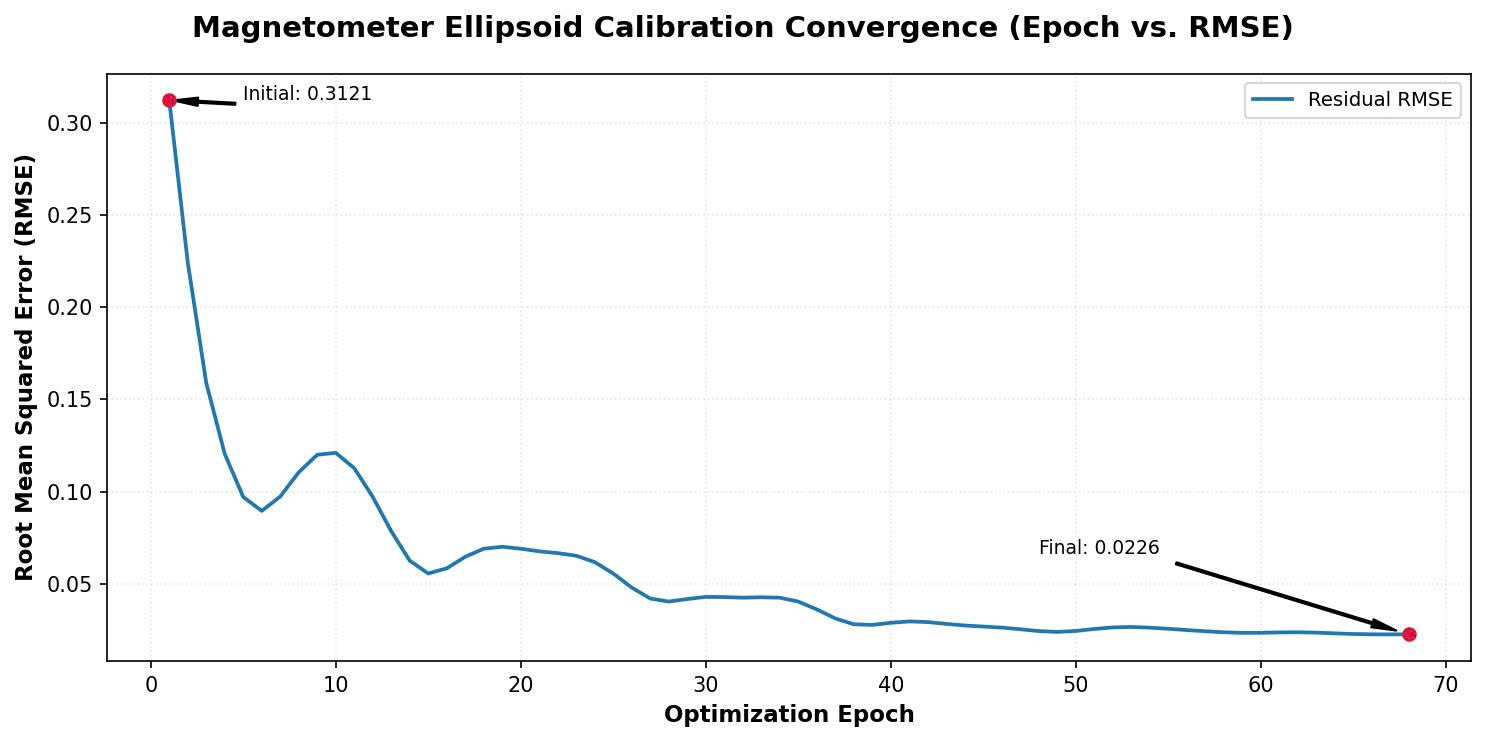
\includegraphics[width=\linewidth]{imgs/mag_calib_convergence.jpg}
\caption{Hội tụ của bộ tối ưu Adam trong hiệu chuẩn ellipsoid từ kế: sai số dư RMSE giảm từ 0.3121 (epoch 0) về 0.0226 (epoch 67).}
\label{fig:ekf-calib}
\end{figure}

\begin{figure}[H]
\centering
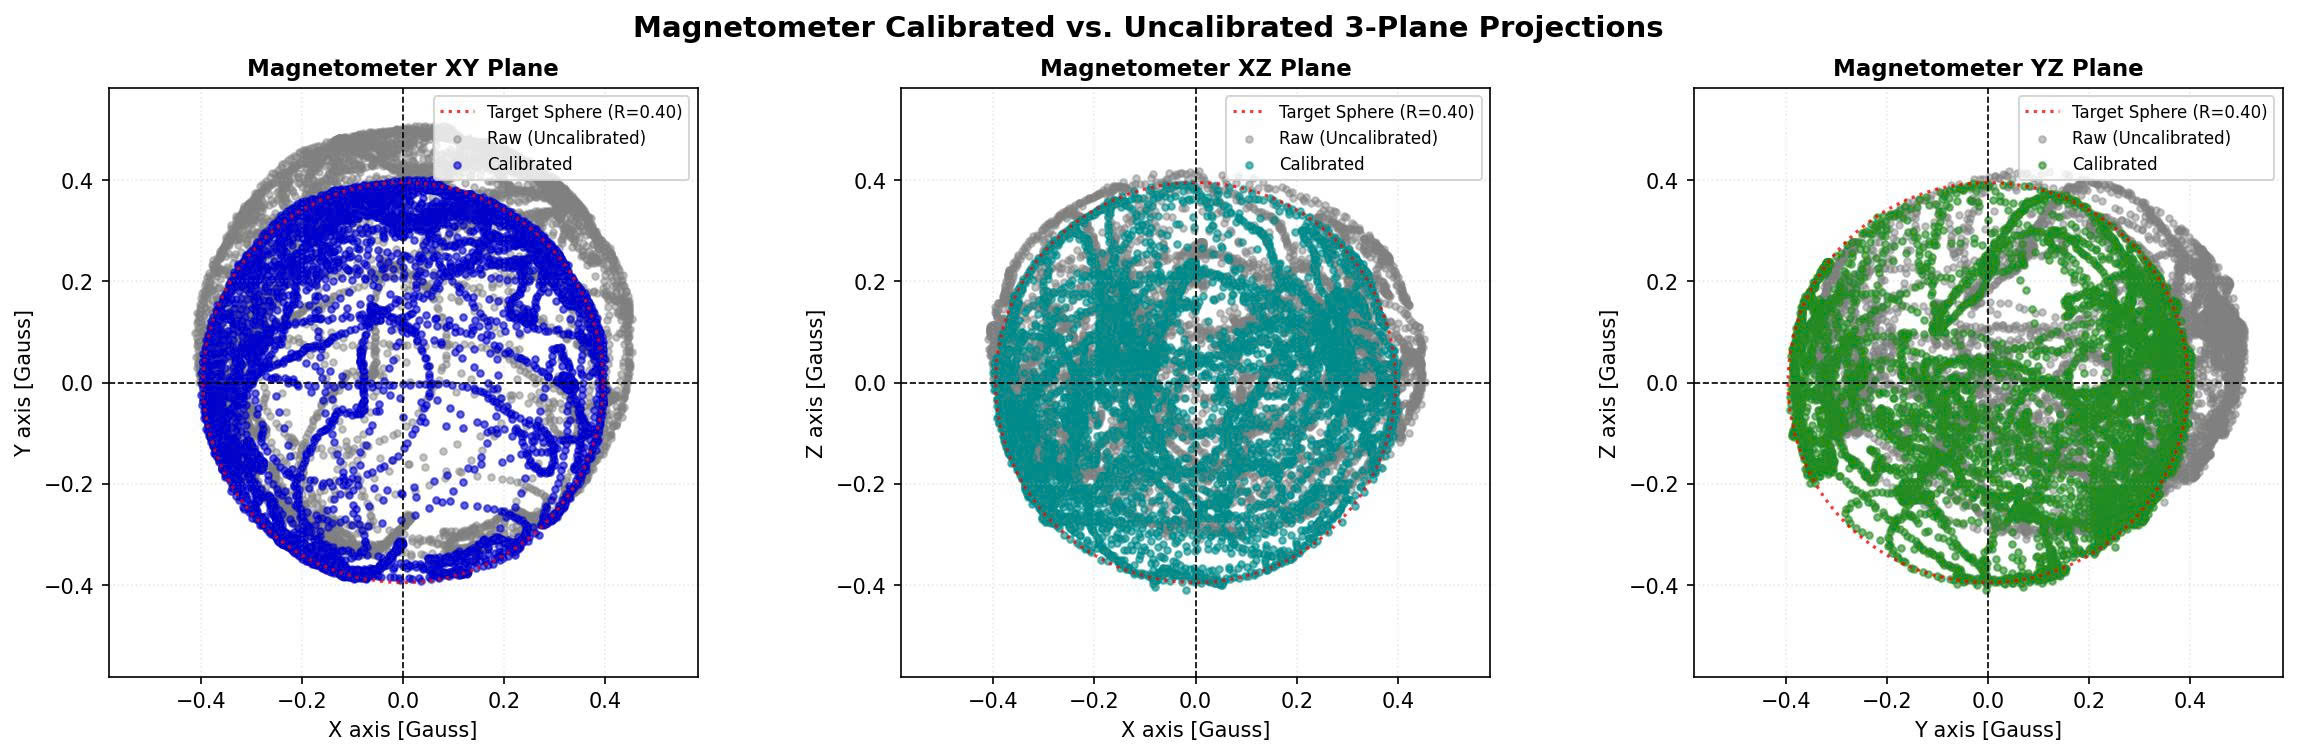
\includegraphics[width=\linewidth]{imgs/mag_calib_projections.jpg}
\caption{Ba phép chiếu mặt phẳng của dữ liệu từ kế trước (xám) và sau (màu) hiệu chuẩn, so với mặt cầu đích bán kính 0.40~Gauss (đường chấm đỏ). Tập điểm hiệu chuẩn bám sát mặt cầu trên cả ba mặt phẳng.}
\label{fig:ekf-calib-proj}
\end{figure}

\subsection{Lọc thông thấp tiền xử lý (Preprocessing Low-Pass Filters)}

Trước khi vào bộ lọc, ba dòng tín hiệu được lọc thông thấp (low-pass filter, LPF): con quay qua LPF bậc hai với tần số góc cắt $\omega_n = 50$~rad/s, gia tốc kế qua LPF bậc một 30~Hz, và từ kế qua LPF bậc một 10~Hz kèm bước chuẩn hóa độ lớn $|\mathbf{m}| = 1$ (ADR~0008). Các tần số cắt được chọn lớn hơn dải tần động của chuyển động độ bay nhưng nhỏ hơn dải nhiễu dao động của khung máy bay, giúp giảm nhiễu đầu vào mà không làm trễ tín hiệu có ích.
